\section{Discussion of HRDNUT Latch} \label{Proposed}

This section discusses the HRDNUT latch. The HRDNUT latch is based on a basic storage block given in Fig. \ref{Block} which contains a 3-input C-element connected to an inverter. This design is derived from a standard keeper element. In addition, the C-element contains two transistors driven by CLK and CLKB. The purpose of the transistors are to set the output to high impedance during the transparent mode. As demonstrated by the DONUT-M, the addition of these transistors drastically reduces the power and delay at a cost of area. Once in the transparent mode, the output is loaded using a pass-gate which allows $D$ to be set directly.     

\begin{figure}[h]
	\centering
	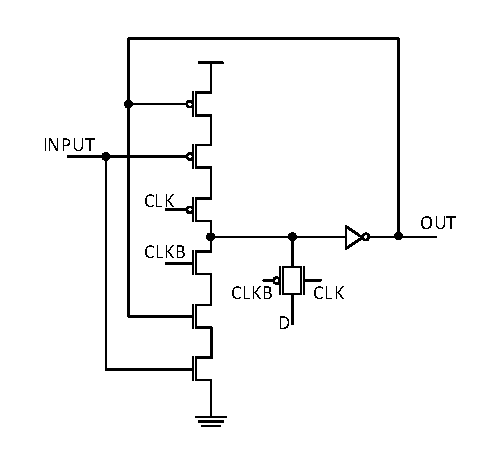
\includegraphics[width=0.5\linewidth]{Figures/Block}
	%where an .eps filename suffix will be assumed under latex, 
	%and a .pdf suffix will be assumed for pdflatex; or what has been declared
	%via \DeclareGraphicsExtensions.
	\caption{Basic data storage loop block.}
	\label{Block}
\end{figure} 

The basic block is then inter-connected to form the block based latch in Fig. \ref{BLatch}. To ensure that the nodes recover after an error, each C-element in the data loop is driven by the other two nodes. This type of configuration ensures that an error on a C-element output is not held. The latch in Fig. \ref{BLatch} is SEU tolerant and DNU tolerant when one error strikes the output C-element. While this latch is not DNU tolerant, it forms the basis for the DNU robust design. To demonstrate the functionality of the latch, we will first describe its operation during normal operation.

In normal operation, the latch data is loaded during the transparent mode. In this mode the input clock \textit{CLK} is high and the inverted clock, \textit{CLKB}, is low. At this stage, nodes \textit{n1}, \textit{n2} and \textit{n3} are set to high impedance and each pass gate is activated allow the value at \textit{D} to be loaded to the corresponding node. Once loaded, the data will propagate to the inputs of the output C-element. During the hold mode, \textit{CLK} is set to a low value and \textit{CLKB} is set high. The held data is reinforced by C-elements \textit{C1}, \textit{C2} and \textit{C3}. The output is then set since the inputs of the output C-element are unanimously held the a single value.

In the case of an SEU in an internal node on the block based latch, the error will propagate to the other C-elements. However, since each C-element has at least one unaffected node, the data on the node will fully recover allowing full recovery of the latch state. In the case of a DNU on the internal nodes, the inputs of the unaffected C-element will be flipped due to the errors. This will ultimately flip the output leading to an error on the output. While this latch is not DNU tolerant, as stated before, it forms the basis for the HRDNUT.

\begin{figure}[!htbp]
	\centering
	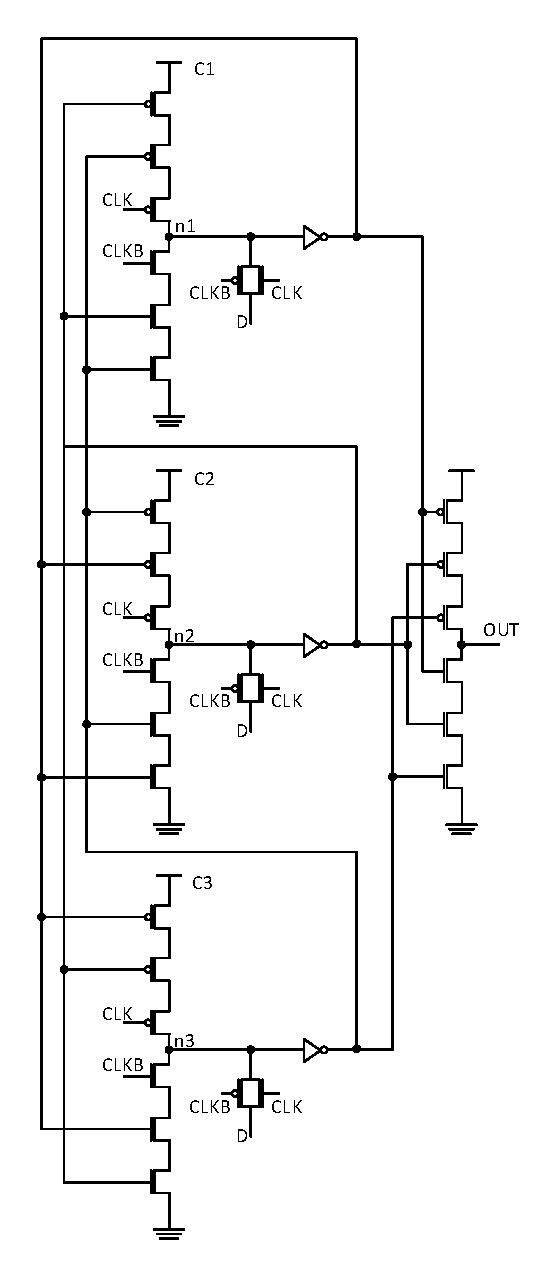
\includegraphics[width=0.55\linewidth]{Figures/BLatch}
	%where an .eps filename suffix will be assumed under latex, 
	%and a .pdf suffix will be assumed for pdflatex; or what has been declared
	%via \DeclareGraphicsExtensions.
	\caption{Schematic of the block-based latch.}
	\label{BLatch}
\end{figure} 

Based on the block latch, the HRDNUT is modified such that no C-element drives itself. More specifically, we first add additional resiliency to the latch by transforming the inverter on node \textit{n2} to a two-input C-element. The second input on this element is driven by the output. This allows for an error on \textit{n2} to be blocked by C-element \textit{C4}. Next, to add resiliency to nodes \textit{n1} and \textit{n3}, elements \textit{C5} and \textit{C6} are added. In addition to DNU tolerance, the C-elements allow for robustness of the latch by ensuring that \textit{C1}, \textit{C2} and \textit{C3} do not drive themselves. Note that on \textit{C5} and \textit{C6}, one NMOS and one PMOS transistor is driven by \textit{OUT} and \textit{n2}. This ensures that the latch will recover all nodes since the node \textit{n5} drives the PMOS on \textit{C7} while the output of \textit{C7} drives the PMOS  on \textit{C5}. The idea behind this is that \textit{n5} only affects C-element \textit{C7} if \textit{n5} is a low value. However, an error on \textit{OUT} does not prevent recovery since \textit{C7} is only affected if \textit{n5} is 0. \textit{C6} operates similarly but node \textit{OUT} drives a NMOS.

Now that we have explained the design process, we will evaluate the HRDNUT latch during normal operation as in \cite{Watkins2016}. When the positive clock signal (CLK) has a high value and the negative clock signal (CLKB) has a low value, the latch is in transparent mode. At this stage, the transistors connected to the clock signal in C-element \textit{C1} deactivates the PMOS and NMOS stacks thus causing the node \textit{n1} to be in a high impedance state. This, in effect, reduces data contention thus reducing delay and dynamic power consumption. Next, the data is loaded through the pass gates connected to nodes \textit{n1}, \textit{n22} and \textit{out}. Since the output node \textit{out} is loaded directly, the data to output delay is minimized and all nodes are set to their respective error free values. When CLK changes to a low value and CLKB to a high value, the latch moves into the hold mode. In this stage, the pass gates are deactivated and the state of the latch is held since each node is driven to the correct value using a C-element. Fig. \ref{NormOp} provides the waveforms of the CLK, D and OUT nodes for both the transparent and hold modes of operation.

\begin{figure}[!htbp]
	\centering
	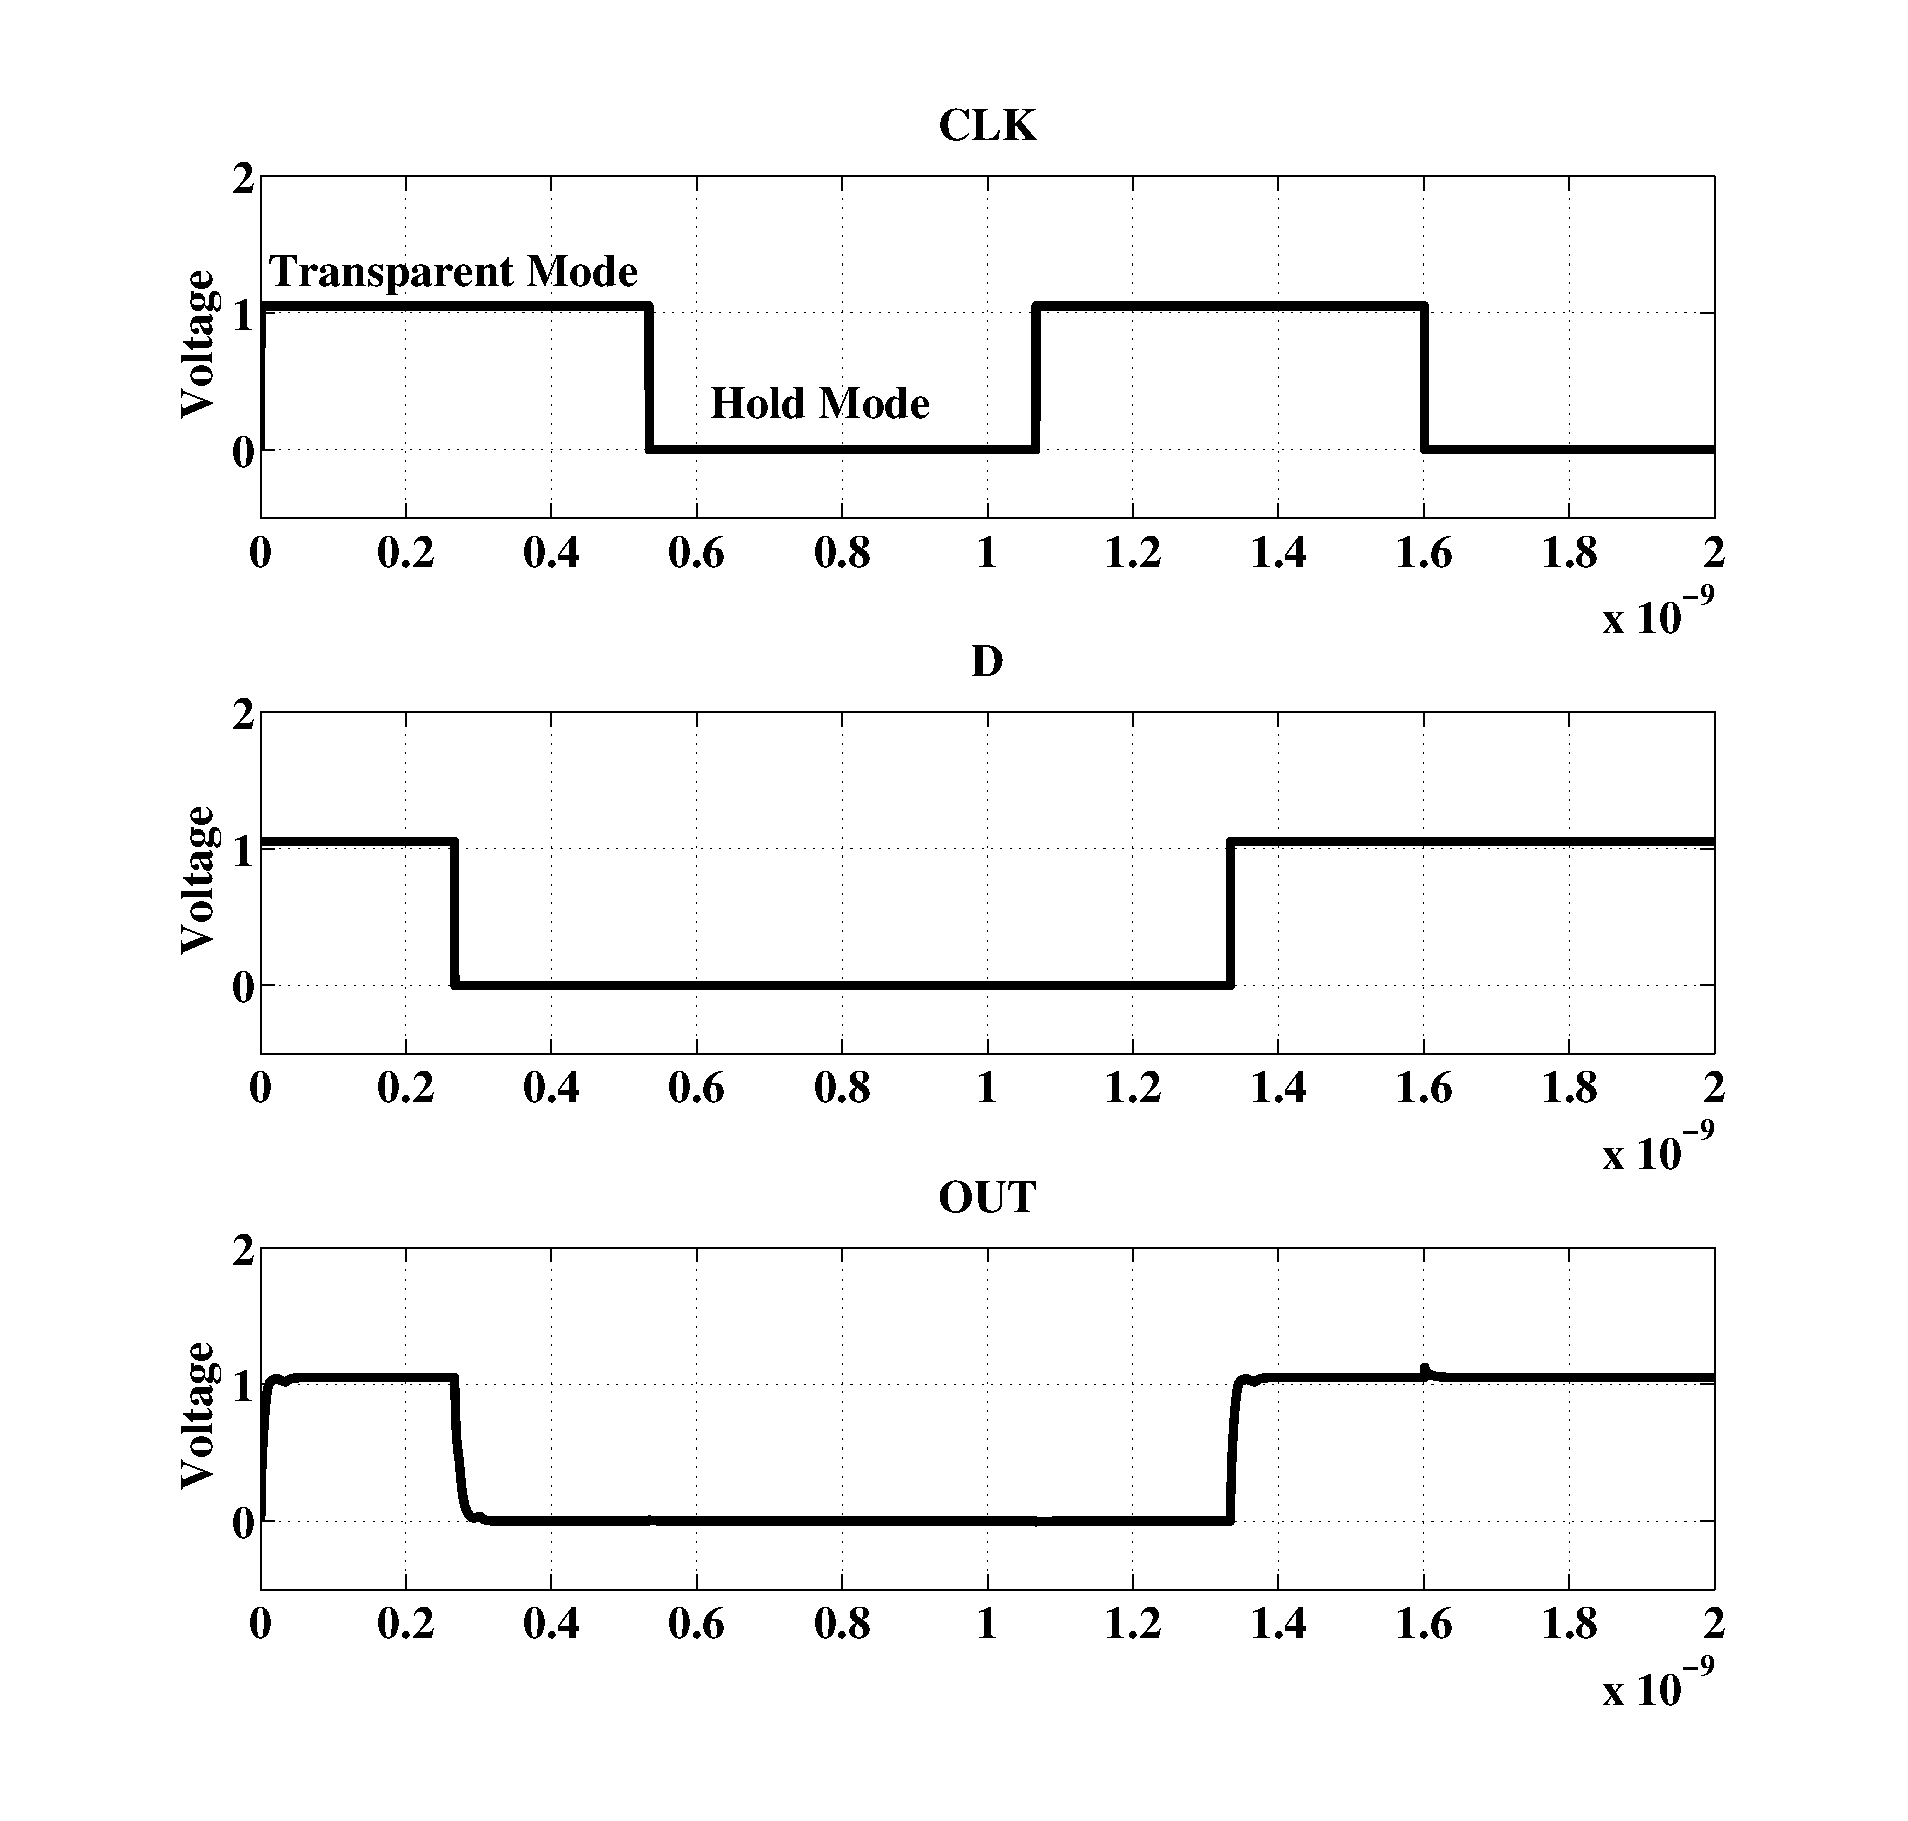
\includegraphics[width=0.80\linewidth]{Figures/defaultoperation.eps}
	%where an .eps filename suffix will be assumed under latex, 
	%and a .pdf suffix will be assumed for pdflatex; or what has been declared
	%via \DeclareGraphicsExtensions.
	\caption{Waveforms of the HRDNUT latch during normal operation.}
	\label{NormOp}
\end{figure}

In the case of an SEU, the HRDNUT retains the SEU resiliency of the block based latch and adds the ability to recover every node after an error. In the case of any internal node being struck by an error, the latch will not change value due to all internal C-elements requiring at least 2 identical input values to change values. In the case of an error hitting the output node \textit{out}, the latch fully recovers since \textit{out} does not directly drive C-element \textit{C7}.

\begin{figure}[!tbp]
	\centering
	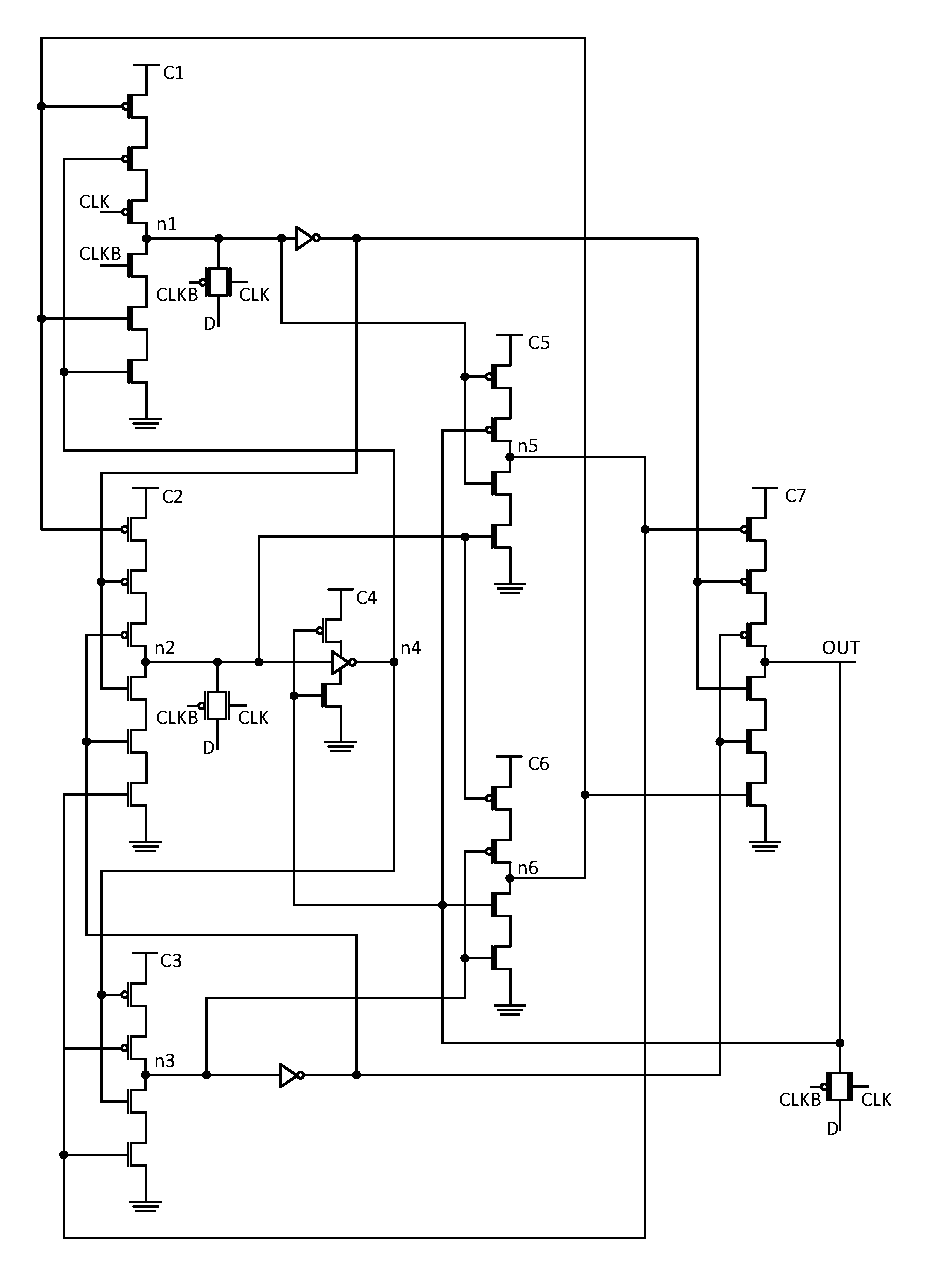
\includegraphics[width=\linewidth]{Figures/HRDNUT}
	%where an .eps filename suffix will be assumed under latex, 
	%and a .pdf suffix will be assumed for pdflatex; or what has been declared
	%via \DeclareGraphicsExtensions.
	\caption{Schematic of the HRDNUT latch.}
	\label{HRDNUT}
\end{figure} 

Lastly, we will evaluate the latch in the case of a DNU. Note that unless otherwise stated, it is assumed that the analysis applies to both when D=0 and D=1. For our analysis, we categorize the possible DNU strike combinations into 9 distinct cases based on their effect in the HRDNUT latch. The categories are discussed in detail below. 

\begin{enumerate}
	\item Consider strikes at nodes \textit{n1} and \textit{n2}. In this case, the error at \textit{n1} will propagate to C-elements \textit{C5} and \textit{C7} but will not cause a flip since the error at \textit{n2} will be blocked by C-element \textit{C4}. Additionally, since the inputs of C-elements \textit{C1} and \textit{C2} are unchanged, the nodes will recover their initial values. This analysis can be applied to node combinations containing node \textit{n2} except for the combination with node \textit{out} since the error will be blocked by C-element \textit{C4}.
	
	\item In the case of a DNU upsetting nodes \textit{n2} and \textit{out}, the error at \textit{n2} will propagate through C-element \textit{C4}. However, C-elements \textit{C1} and \textit{C3} will block the error and nodes \textit{n1}, \textit{n3}, \textit{n5} and \textit{n6} will hold their values thus driving node \textit{out} to the correct state. 

	\item Consider when a DNU strikes nodes \textit{n1} and \textit{n5}. In this case, the error at \textit{n1} hits the output of C-element \textit{C1} which is propagated to \textit{C7}. The error on \textit{n5} is also propagated to C-element \textit{C7}. Since node \textit{n3} and the inputs of C-elements \textit{C1} and \textit{C5} are unaffected by an error, the output retains the error-free value and the latch fully recovers the previous state. The above analysis also applies to the node combination (\textit{n3}, \textit{n6}).

	\item In the case of a DNU hitting nodes \textit{n3} and \textit{n4}, the error at \textit{n4} is propagated to C-element \textit{C3} and the error at \textit{n3} is propagated to \textit{C7} and \textit{C6}. After the error on \textit{n3} subsides, \textit{C4} will drive node \textit{n4} and, due to the connection at \textit{C3}, node \textit{n3} back to the error-free value. The node combination (\textit{n1}, \textit{n1}) can be analyzed similarly. For the node combinations of (\textit{n4}, \textit{n5}) and (\textit{n4}, \textit{n6}), the latch will also recover the previous result since the inputs to \textit{C4} are unchanged. This implies that after the error occurs at \textit{n4}, the node will be driven back to the correct value thus also driving the nodes \textit{n5} or \textit{n6} back to the correct value.
	
	\item When a DNU upsets the combination of \textit{n4} and \textit{out}, the error at \textit{out} is propagated to \textit{C4}, \textit{C5} and \textit{C6} and the error at \textit{n4} to \textit{C1} and \textit{C3}. Since none of the inputs to \textit{C7} are changed by the error, \textit{out} is flipped back to its error-free value which drives \textit{n4} through \textit{C4} back to its previous state.

	\item Consider when a DNU strikes nodes \textit{n1} and \textit{n3} being struck. In this case, the errors are propagated to C-elements \textit{C2}, \textit{C5}, \textit{C6} and \textit{C7}. However, since the errors do not manifest into an error on any other node, the latch fully recovers from the error. 
	
	\item When a DNU strikes the nodes \textit{n1} and \textit{n6}. The error at node \textit{n6} propagates to  \textit{C1} and \textit{C7} while the error at \textit{n1} also propagates to \textit{C7}. Due to the error-free node \textit{n3} driving \textit{C7}, the previous value is held at the output by \textit{C7}. Additionally, \textit{n3} will drive \textit{C6} back to its previous value thus driving \textit{C1} back to the error free state. This analysis can be applied similarly to the node combination of (\textit{n3}, \textit{n5}). 

	\item In the case where a DNU strikes nodes \textit{n5} and \textit{out}, the error at \textit{n5} propagates to \textit{C7}, \textit{C2} and \textit{C3} and the error at \textit{out} goes to \textit{C4}, a PMOS in \textit{C5}, and a NMOS in \textit{C6}. When the error-free value at \textit{out} is 1, the value at \textit{n5} is 0. The error at the nodes change the values to 0 and 1, respectively, and the erroneous value at \textit{out} is propagated to the PMOS at \textit{C5} and the NMOS at \textit{C6}. This, in effect, causes the PMOS at \textit{C5} to be activated and the NMOS at \textit{C6} to be deactivated. However, since nodes \textit{n1} and \textit{n2} remain error-free, the NMOS stack of \textit{C5} will drive \textit{n5} back to the correct value. This, in turn, forces \textit{C7} to also drive \textit{out} back to the error-free value. In the case where \textit{out} has an ideal value of 0, the error will be fully recovered since the NMOS stack will be entirely driven by fault-free nodes. The above analysis can be applied to the node combination of (\textit{n6}, \textit{out}). 
	
	\item Lastly, we analyze the node combinations (\textit{n1}, \textit{out}), (\textit{n3}, \textit{out}) and (\textit{n5}, \textit{n6}). In these cases the errors do not cause a change on the inputs of any C-elements driving the node thus the previous value will always be recovered. 
\end{enumerate}

To evaluate the design, pulses were injected using the equation given in \cite{injeq}. The equation is given below with $\tau$ as the technology dependent constant, $Q_o$ as the injection current value and $t$ as the variable for time. In the equation $\tau$ was set to $32\times10^{-12}$ and $Q_o$ was set to $5\text{fC}$. The result of this simulation for each distinct case is given in Figs. \ref{fig:CLK}-\ref{fig:n5n6}, respectively. 

\begin{equation}\label{qeq}
	I(t)=\frac{2Q_o}{\tau\sqrt{\pi}}\sqrt{\frac{t}{\tau}}e^{\frac{-t}{\tau}}
\end{equation}

\begin{figure}[!htbp]
	\centering
	\parbox{4cm}{
		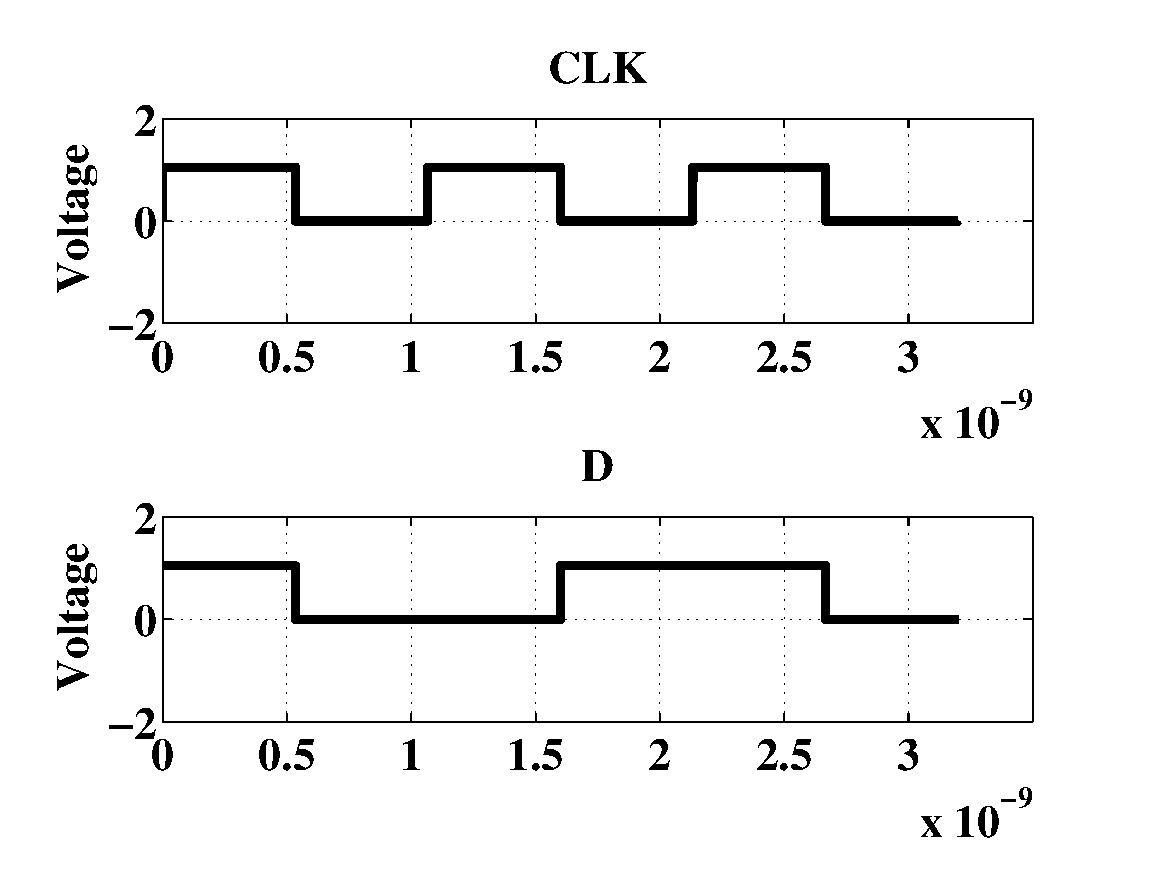
\includegraphics[width=1.15\linewidth]{Figures/WavePlots/CLKD.eps}
		\caption{Waveforms for CLK and D.}
		\label{fig:CLK}}
	\qquad
	\begin{minipage}{4cm}
		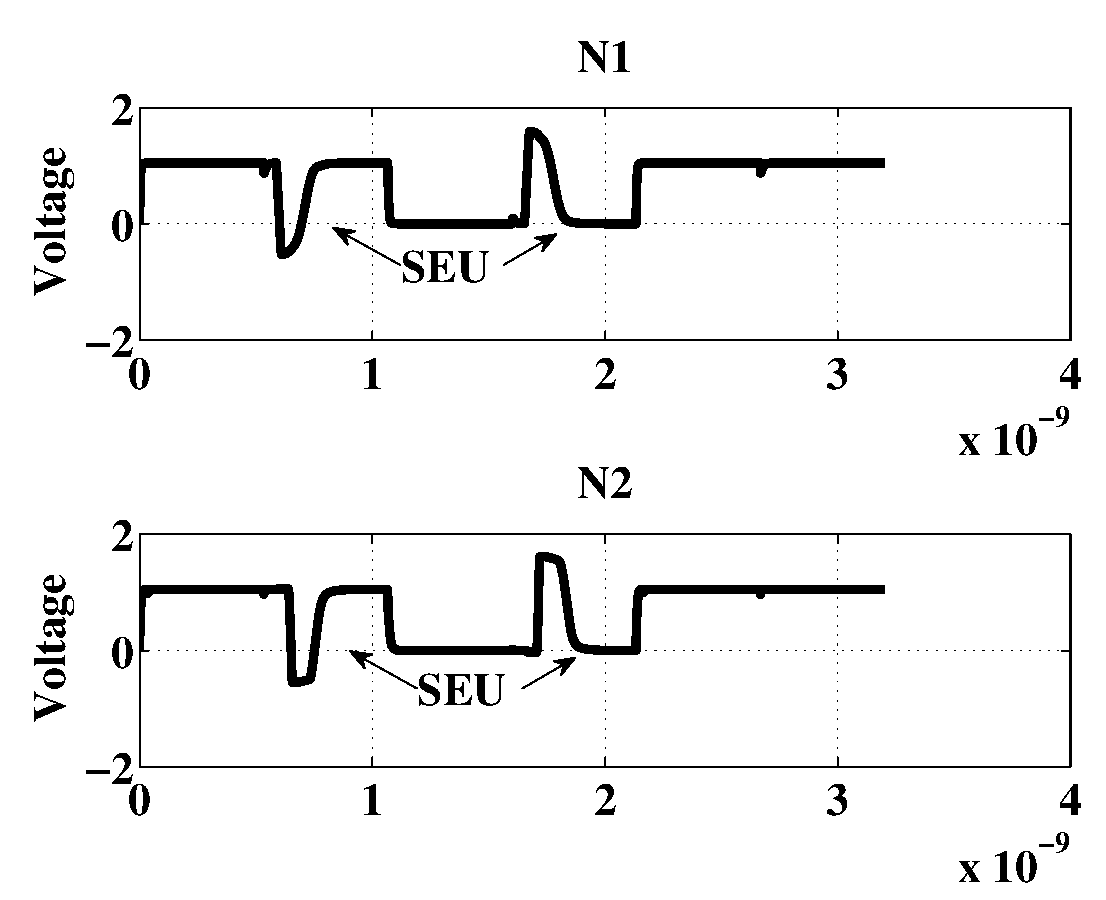
\includegraphics[width=\linewidth]{Figures/WavePlots/n1n2.eps}
		\caption{Node pair n1 and n2 upset and recovery.}
		\label{fig:n1n2}
	\end{minipage}
\end{figure}

\begin{figure}[!htbp]
	\centering
	\parbox{4cm}{
		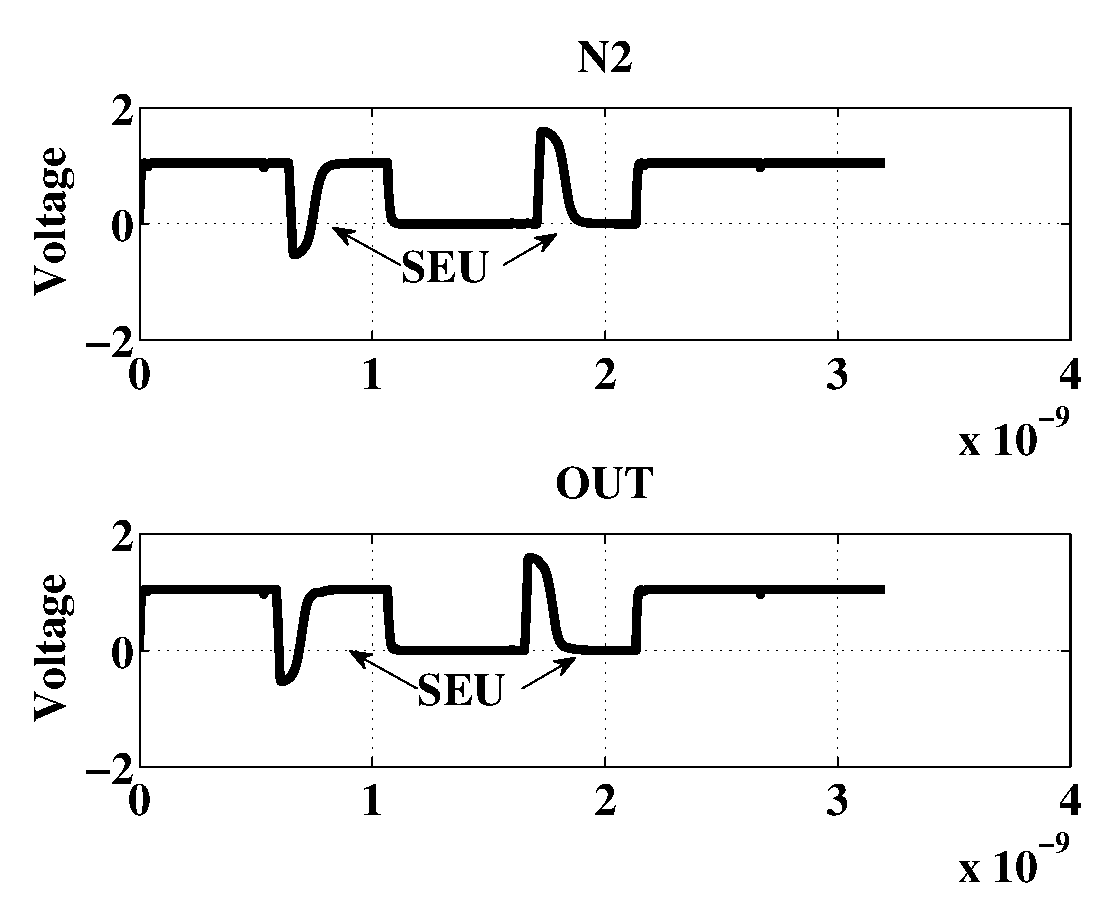
\includegraphics[width=\linewidth]{Figures/WavePlots/n2out.eps}
		\caption{Node pair n2 and out upset and recovery.}
		\label{fig:n2out}}
	\qquad
	\begin{minipage}{4cm}
		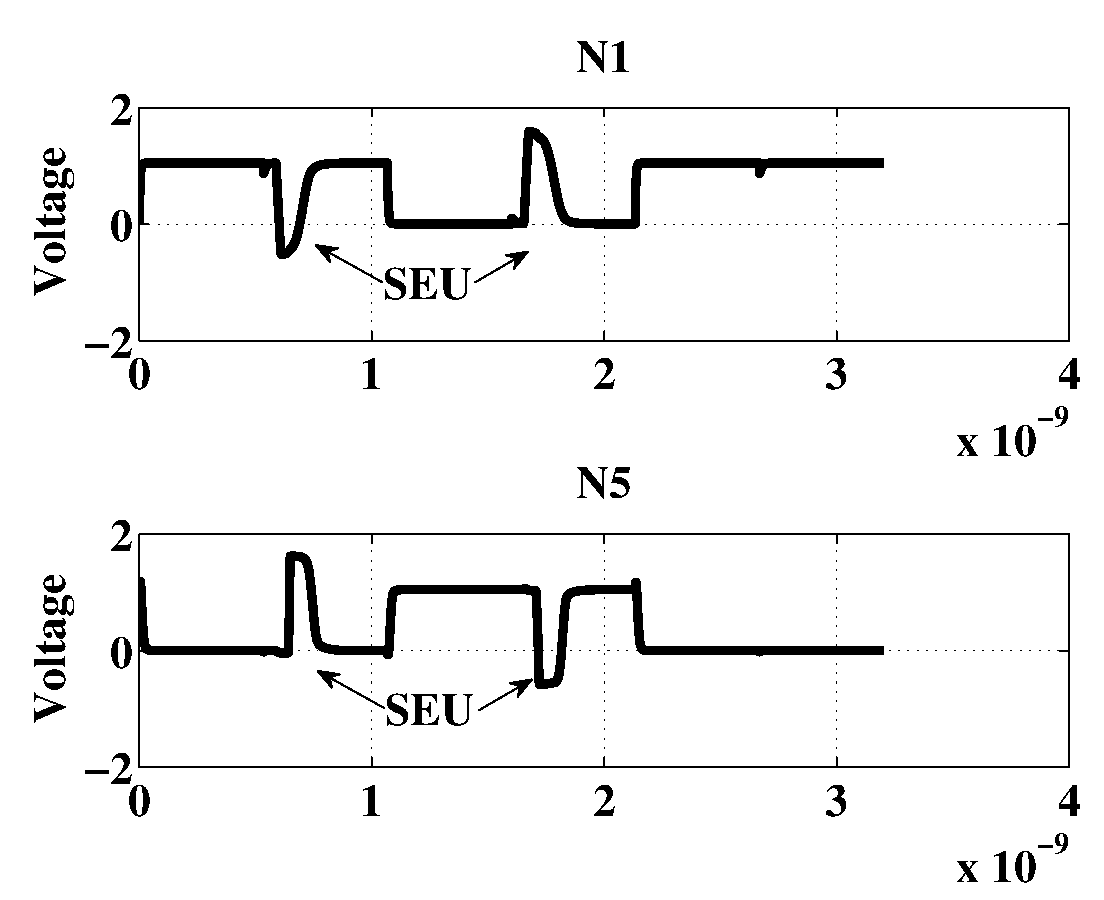
\includegraphics[width=\linewidth]{Figures/WavePlots/n1n5.eps}
		\caption{Node pair n1 and n5 upset and recovery.}
		\label{fig:n1n5}
	\end{minipage}
\end{figure}

\begin{figure}[!htbp]
	\centering
	\parbox{4cm}{
		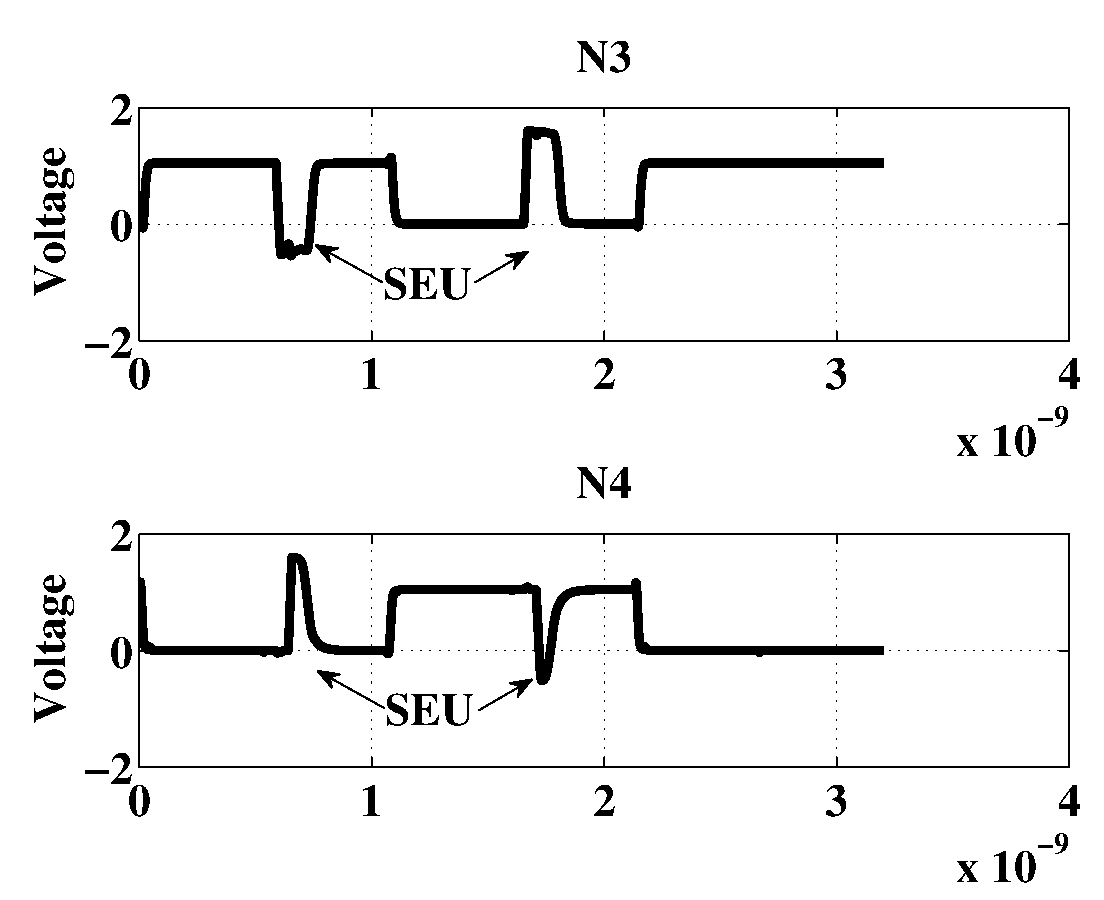
\includegraphics[width=\linewidth]{Figures/WavePlots/n3n4.eps}
		\caption{Node pair n3 and n4 upset and recovery.}
		\label{fig:n3n4}}
	\qquad
	\begin{minipage}{4cm}
		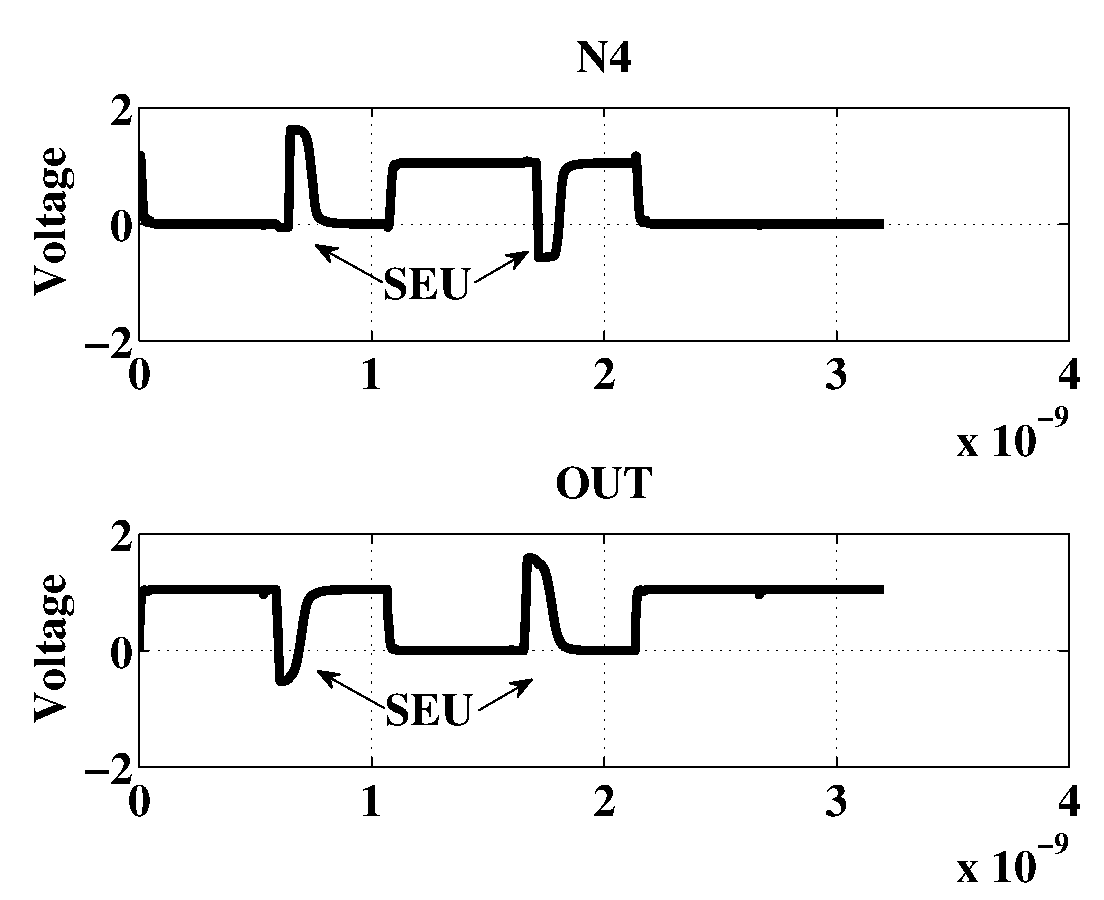
\includegraphics[width=\linewidth]{Figures/WavePlots/n4out.eps}
		\caption{Node pair n4 and out upset and recovery.}
		\label{fig:n4out}
	\end{minipage}
\end{figure}

\begin{figure}[!htbp]
	\centering
	\parbox{4cm}{
		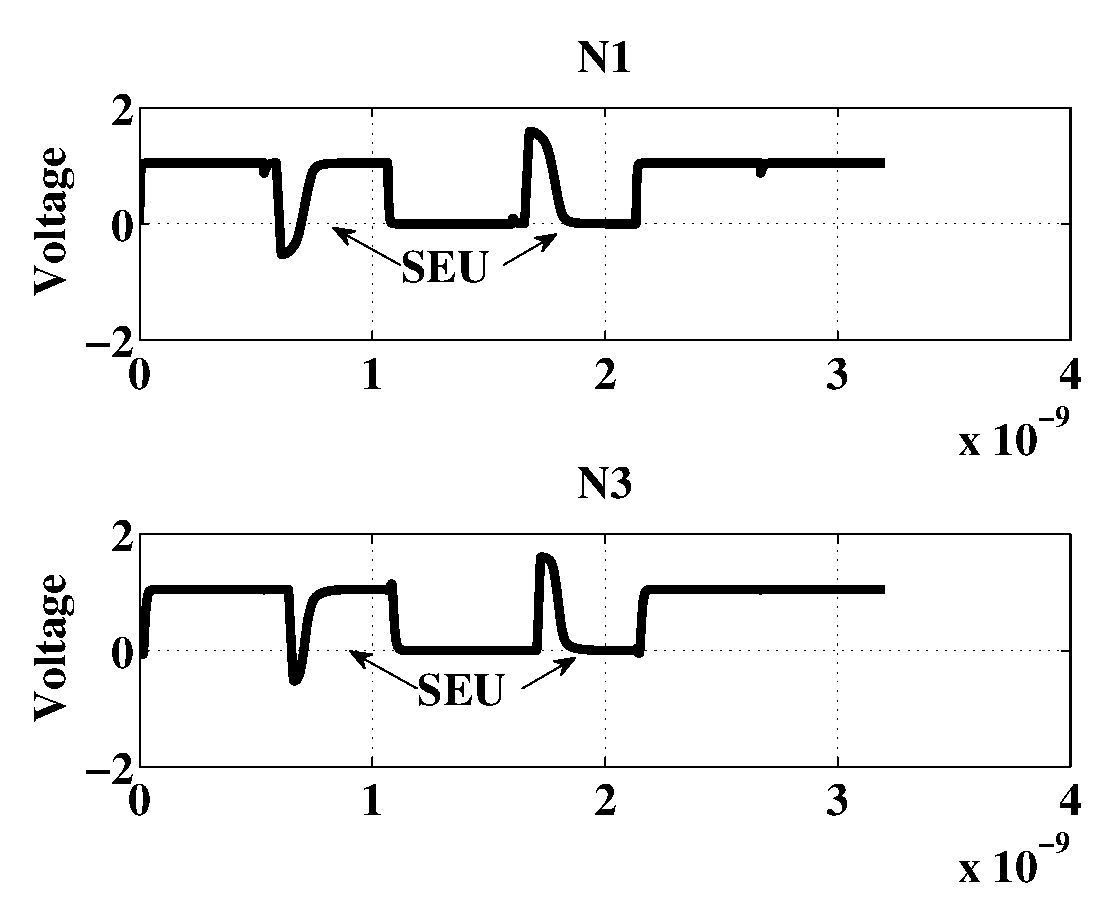
\includegraphics[width=\linewidth]{Figures/WavePlots/n1n3.eps}
		\caption{Node pair n1 and n3 upset and recovery.}
		\label{fig:n1n3}}
	\qquad
	\begin{minipage}{4cm}
		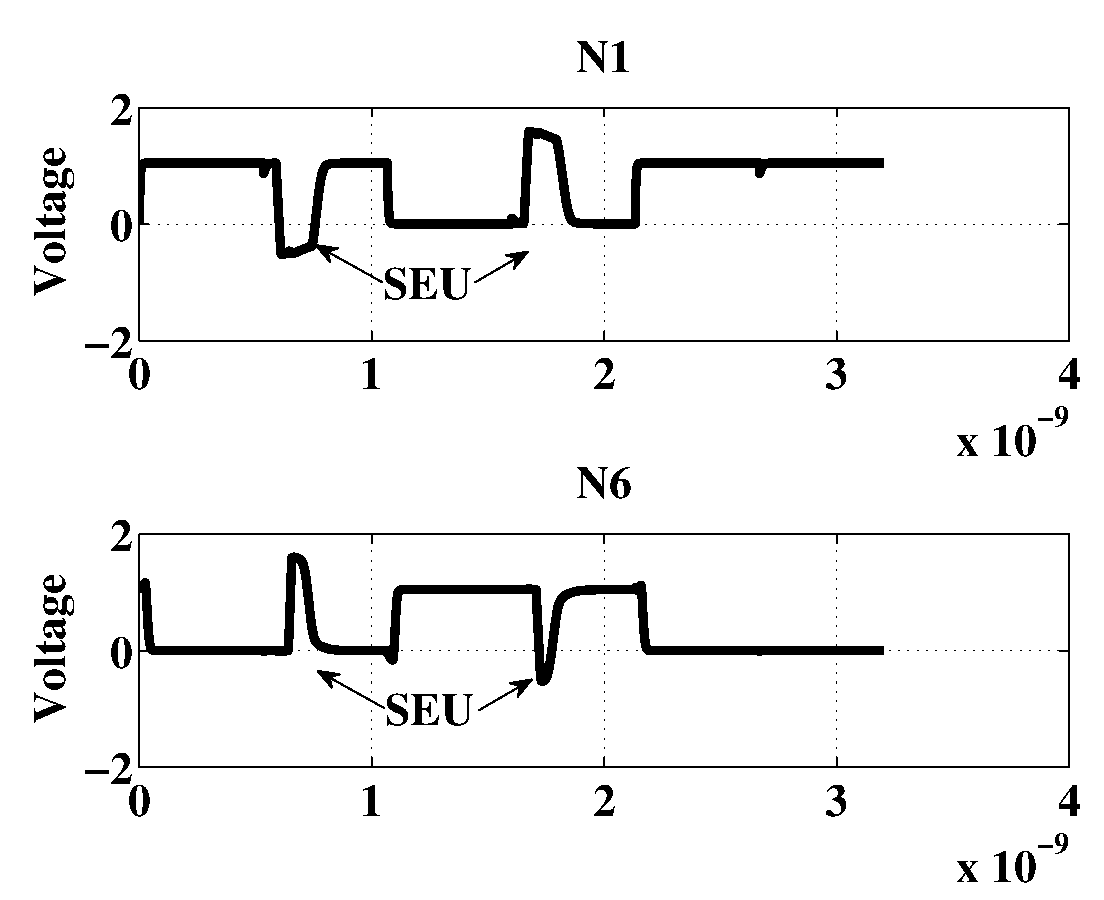
\includegraphics[width=\linewidth]{Figures/WavePlots/n1n6.eps}
		\caption{Node pair n1 and n6 upset and recovery.}
		\label{fig:n1n6}
	\end{minipage}
\end{figure}

\begin{figure}[!htbp]
	\centering
	\parbox{4cm}{
		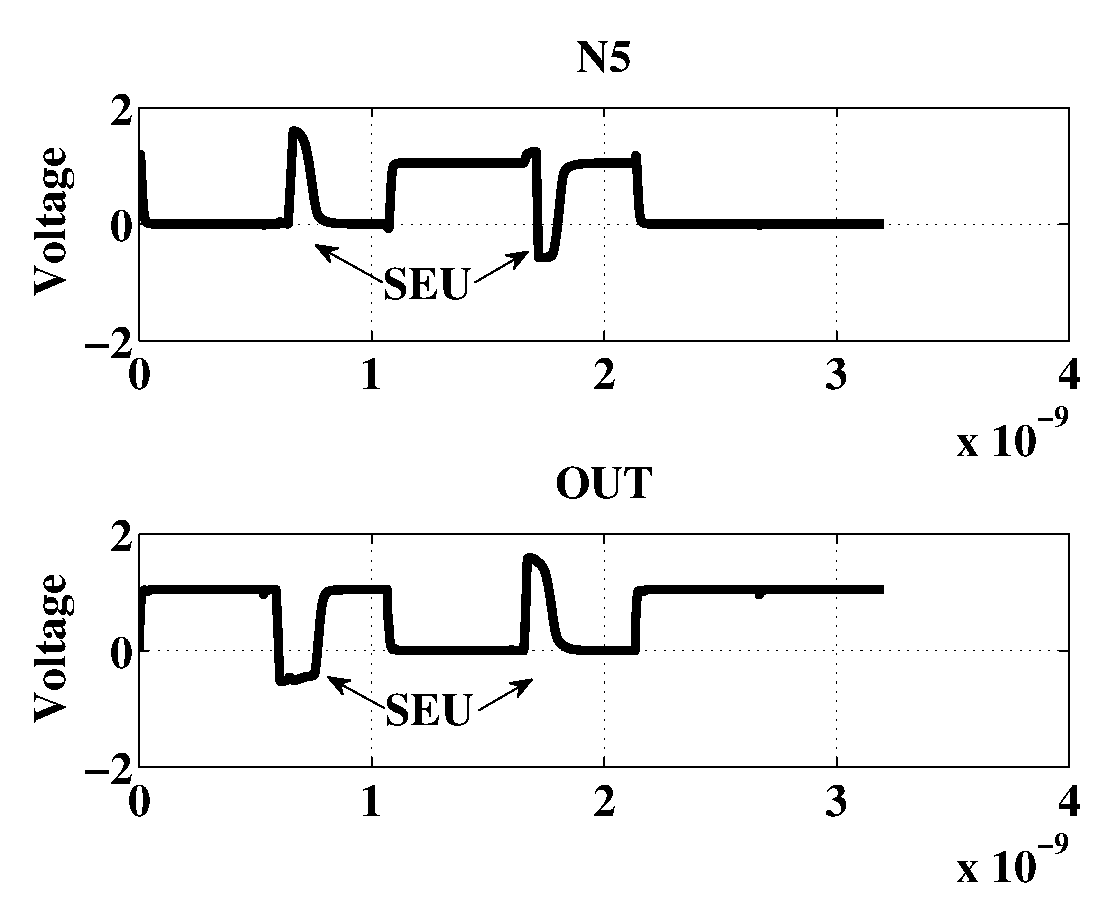
\includegraphics[width=\linewidth]{Figures/WavePlots/n5out.eps}
		\caption{Node pair n5 and out upset and recovery.}
		\label{fig:n3out}}
	\qquad
	\begin{minipage}{4cm}
		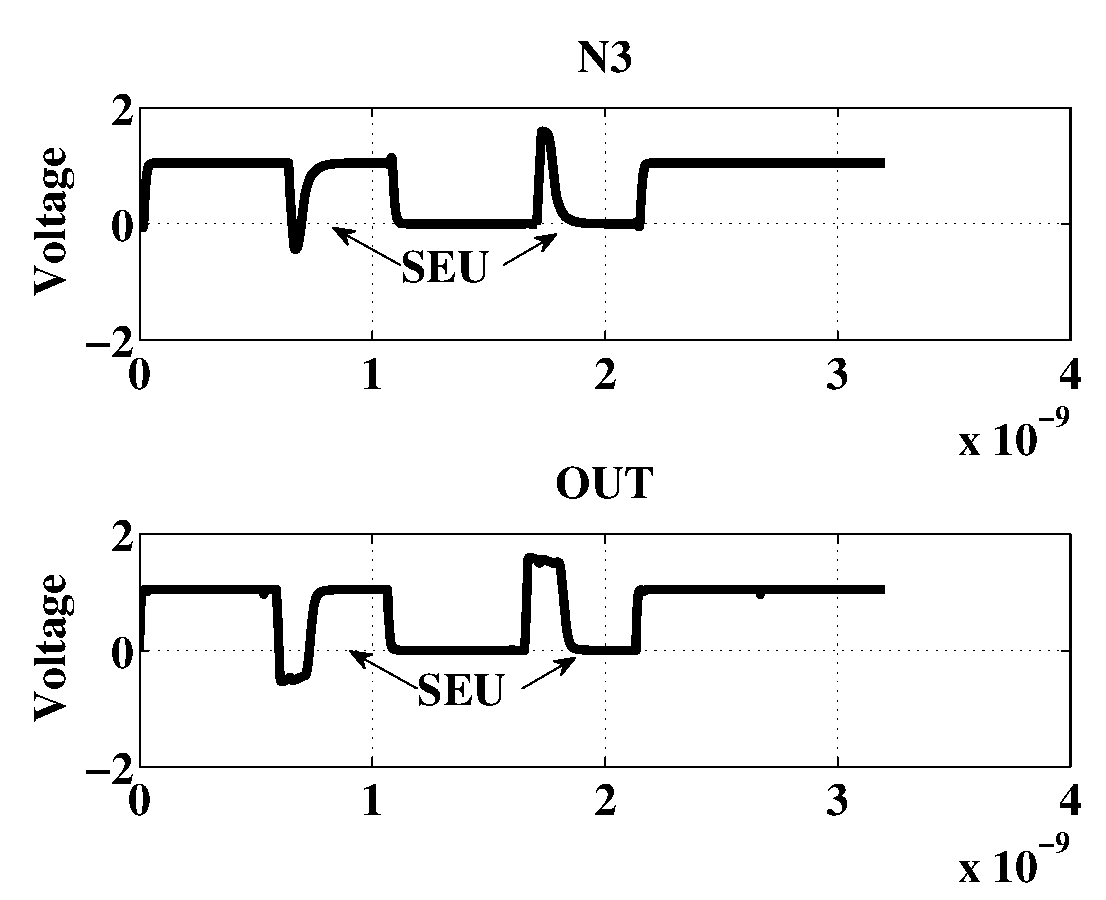
\includegraphics[width=\linewidth]{Figures/WavePlots/n3out.eps}
		\caption{Node pair n3 and out upset and recovery.}
		\label{fig:n5n6}
	\end{minipage}
\end{figure}